\section{Pruebas llevadas a cabo} \label{sec:pru}
% describiranse as probas realizadas aos distintos niveis para
% garantir o correcto funcionamento do software ou do hardware.
    
    Muchos de los paradigmas de programación ágil abarcan el concepto de prueba unitaria. Pruebas programadas en el mismo lenguaje que se escribe la aplicación y que permiten comprobar el funcionamiento de una unidad de código. Sin embargo, dado que desde el inicio del proyecto no estaban claras las fuentes de información que iban a ser utilizadas debido a la gran variedad de librerías y las diferencias entre estas, además de la posibilidad de la adición de cambios en el proyecto que pudiesen cambiar toda su estructura y funcionamiento, se tomó la decisión de no utilizar pruebas automatizadas.
    
    \subsection{Pruebas generales de funcionamiento}
        Para comprobar si el sistema funcionaba correctamente se decidió realizar pruebas manuales, comprobando con cada cambio las funcionalidades previamente desarrolladas. Esto permitiría desarrollar una base del sistema, es decir, alcanzar un punto donde el agente fuese capaz de gestionar correctamente los diferentes \textit{plugins} y hacer uso de estos a través de la \textit{CLI}.
        
    \subsection{Pruebas de funcionamiento como servicio}
        Las pruebas mencionadas anteriormente fueron muy útiles durante el desarrollo de de las funcionalidades principales, sin embargo, probar el servicio supuso una tarea más complicada ya que no era posible mostrar la información en la línea de comandos.
        
        Para comprobar la ejecución del agente al ser utilizado como servició se utilizaron dos métodos, comprobar los sistemas remotos a donde se enviaba la información a ver si llegaba correctamente y los \textit{eventos del sistema} donde se mostraría cualquier información relacionada con el agente en sí.
        
        El desarrollo de un sistema de actualización automática ayudó con las pruebas mencionadas en este apartado, ya que eliminó la necesidad de reiniciar el servicio manualmente y de copiar nuevas versiones de los \textit{plugins} en cada prueba.
    
    \subsection{Pruebas de actualización automática}
        Para comprobar que el sistema de actualización automática funcionara correctamente se utilizaron los \textit{eventos del sistema}, donde se añadirían \textit{logs} para cada acción realizada, como la actualización de algún componente, cualquier tipo de fallo, o un indicador de que el proceso de actualización había terminado.
        
    \subsection{Eventos del sistema}
        Cada \textit{log} creado por el agente o el sistema de actualización automática cuenta con un identificador de evento que permite saber de dónde proviene el mensaje recibido. En el anexo \ref{anx:eventid} se muestra una lista con los identificadores para cada uno de los procesos.
        
    \subsection{Resultados obtenidos}
        En las figuras \ref{fig:rabbitmq-prod-queue} y \ref{fig:rabbitmq-dev-queue} se muestran las colas de dos servidores de \textit{RabbitMQ} (producción y desarrollo), donde se pueden apreciar los resultados de la ejecución como servicio en uno de los servidores \textit{Windows} del \textit{CERN} durante varios días. La configuración utilizada incluye más \textit{plugins} de los inicialmente planteados para este proyecto (\textit{HeartBeat} y \textit{Updates}), los cuales se han mantenido en ejecución por más de una semana.
        
        \begin{figure}[h!]
        \centering
            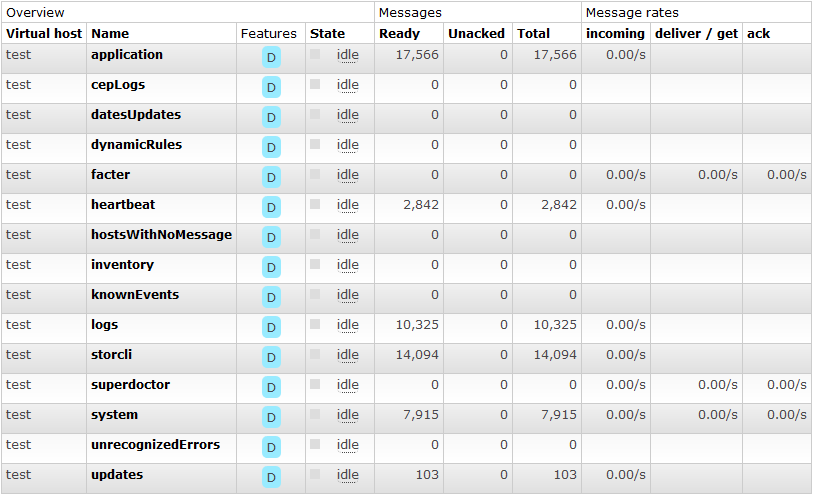
\includegraphics[scale=0.69]{cola-rabbit-mq-prod.png}
            \caption{Colas de RabbitMQ - Producción}
            \label{fig:rabbitmq-prod-queue}
        \end{figure}
    
        \begin{figure}[h!]
        \centering
            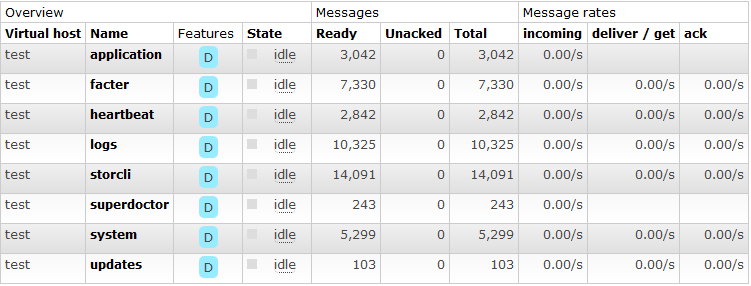
\includegraphics[scale=0.7]{cola-rabbit-mq-dev.png}
            \caption{Colas de RabbitMQ - Desarrollo}
            \label{fig:rabbitmq-dev-queue}
        \end{figure}
        
        Estas imágenes demuestran que hay datos llegando a los servidores \textit{RabbitMQ}, sin embargo, el número de horas de ejecución del agente no coincide con la cantidad de paquetes recibidos para ambos \textit{plugins}. Esto se debe a que la información almacenada en estos servidores incluye mensajes de pruebas anteriores, además de varios reiniciaos del servicio, que hacen que se vuelva a realizar el envío de la información por parte de los \textit{plugins} aunque no haya pasado el tiempo establecido para ello.
        
        En las imágenes \ref{fig:rabbitmq-rate-heartbeat} y \ref{fig:rabbitmq-rate-updates} se pueden apreciar el número de mensajes recibidos en una hora (rango máximo que permiten las gráficas de \textit{RabbitMQ}), esto sí coincide con la configuración aplicada en el servicio, un mensaje de \textit{HeartBeat} cada dos minutos y uno de \textit{Updates} cada una hora.
        
        \begin{figure}[h!]
        \centering
            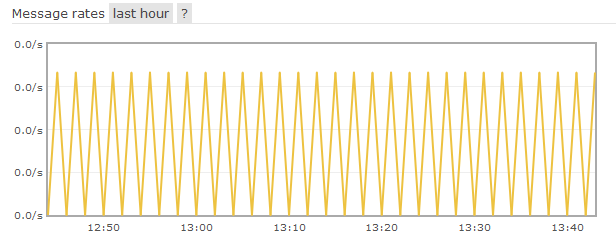
\includegraphics[scale=0.7]{rate-rabbit-mq-heartbeat.png}
            \caption{Mensajes por hora - HeartBeat}
            \label{fig:rabbitmq-rate-heartbeat}
        \end{figure}
        
        \begin{figure}[h!]
        \centering
            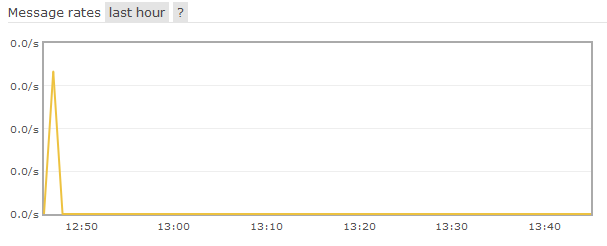
\includegraphics[scale=0.7]{rate-rabbit-mq-updates.png}
            \caption{Mensajes por Hora - Updates}
            \label{fig:rabbitmq-rate-updates}
        \end{figure}
        